Wanneer gekeken wordt naar figuur \ref{tijd} valt meteen op dat \texit{Fast Non-Local Mean Denoising} voor om het even welke kernel grootte niet echt efficiënt is. Dit kon alreeds verwacht worden door de manier waarop deze methode te werk gaat. Het is trager met een orde van grootte 3. Om deze reden zal deze filter al zeker niet opgenomen worden in het project. Verder zijn er nog twee opvallende zaken. Enerzijds zorgt een grotere kernel ervoor dat de \textit{Median filter} veel meer tijd nodig heeft.
\begin{figure}[h]
    \centering
    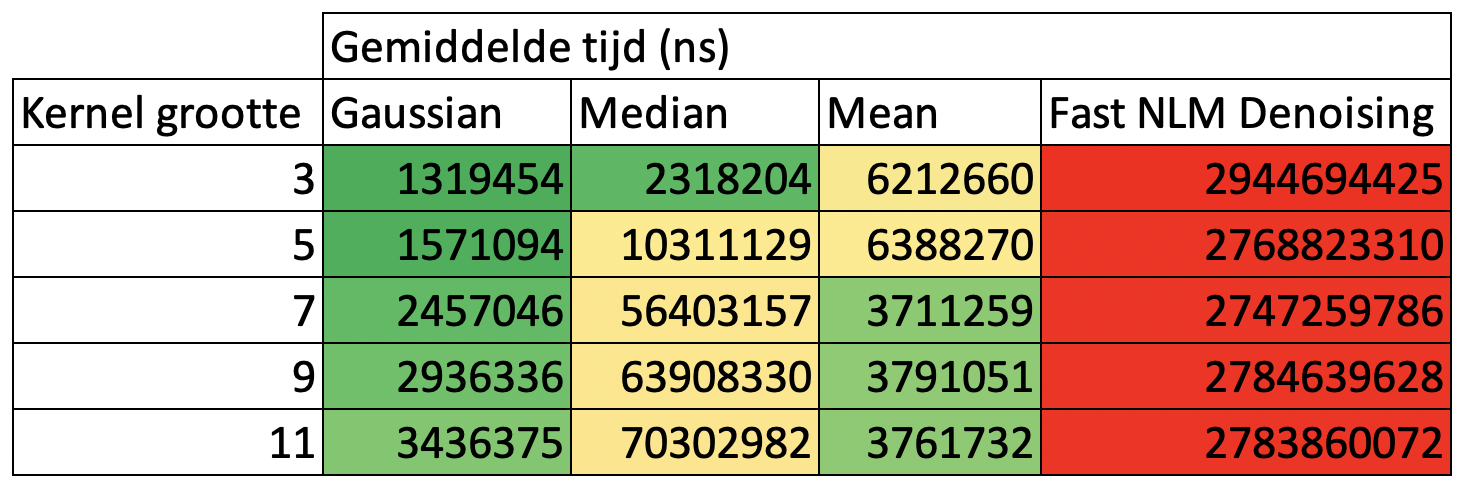
\includegraphics[scale=0.5]{img/tijdsconsumptie}
    \caption{Gemiddelde tijd nodig om filter op afbeelding toe te passen.}
    \label{fig:tijd}
\end{figure}